\section{Results}
\label{sec:results}

We present experimental results from the inference and post-editing tracks, analyze performance patterns, and evaluate the quality-evasion trade-off.

\subsection{Leaderboard Rankings}

Table~\ref{tab:leaderboard} presents the complete leaderboard ranking methods by evasion rate. All methods are evaluated against the same detector ensemble.

\begin{table}[t]
\centering
\caption{Leaderboard ranking of undetectability methods. Methods are ranked by evasion rate (1 - TPR@5\%FPR). Higher evasion rates are better. Quality score represents content preservation (1.0 for inference methods, word overlap for post-editing).}
\label{tab:leaderboard}
\small
\begin{tabular}{@{}clllcccc@{}}
\toprule
\textbf{Rank} & \textbf{Track} & \textbf{Method} & \textbf{AUROC} & \textbf{TPR@5\%} & \textbf{Evasion} & \textbf{Quality} \\
\midrule
1 & Inference & human\_style & 0.79 & 0.30 & \textbf{0.70} & 1.00 \\
2 & Inference & varied & 0.77 & 0.30 & \textbf{0.70} & 1.00 \\
3 & Post-edit & casual\_style & 0.85 & 0.30 & \textbf{0.70} & 0.16 \\
4 & Post-edit & simple\_paraphrase & 0.76 & 0.30 & \textbf{0.70} & 0.42 \\
5 & Inference & personal & 0.83 & 0.40 & 0.60 & 1.00 \\
6 & Inference & baseline & 0.85 & 0.50 & 0.50 & 1.00 \\
7 & Post-edit & baseline & 0.91 & 0.50 & 0.50 & 1.00 \\
8 & Post-edit & personal\_style & 0.97 & 0.70 & 0.30 & 0.18 \\
\bottomrule
\end{tabular}
\end{table}

\paragraph{Key Observations.} The top four methods all achieve 70\% evasion rate, representing a 40\% relative improvement over the 50\% baseline. Notably, two inference methods (human\_style, varied) match the best post-editing methods while preserving full content quality. The personal\_style post-editing method performs worst, achieving only 30\% evasion---worse than doing nothing.

\subsection{Track Comparison}

Figure~\ref{fig:track_comparison} compares the two tracks across detection metrics.

\begin{figure}[t]
    \centering
    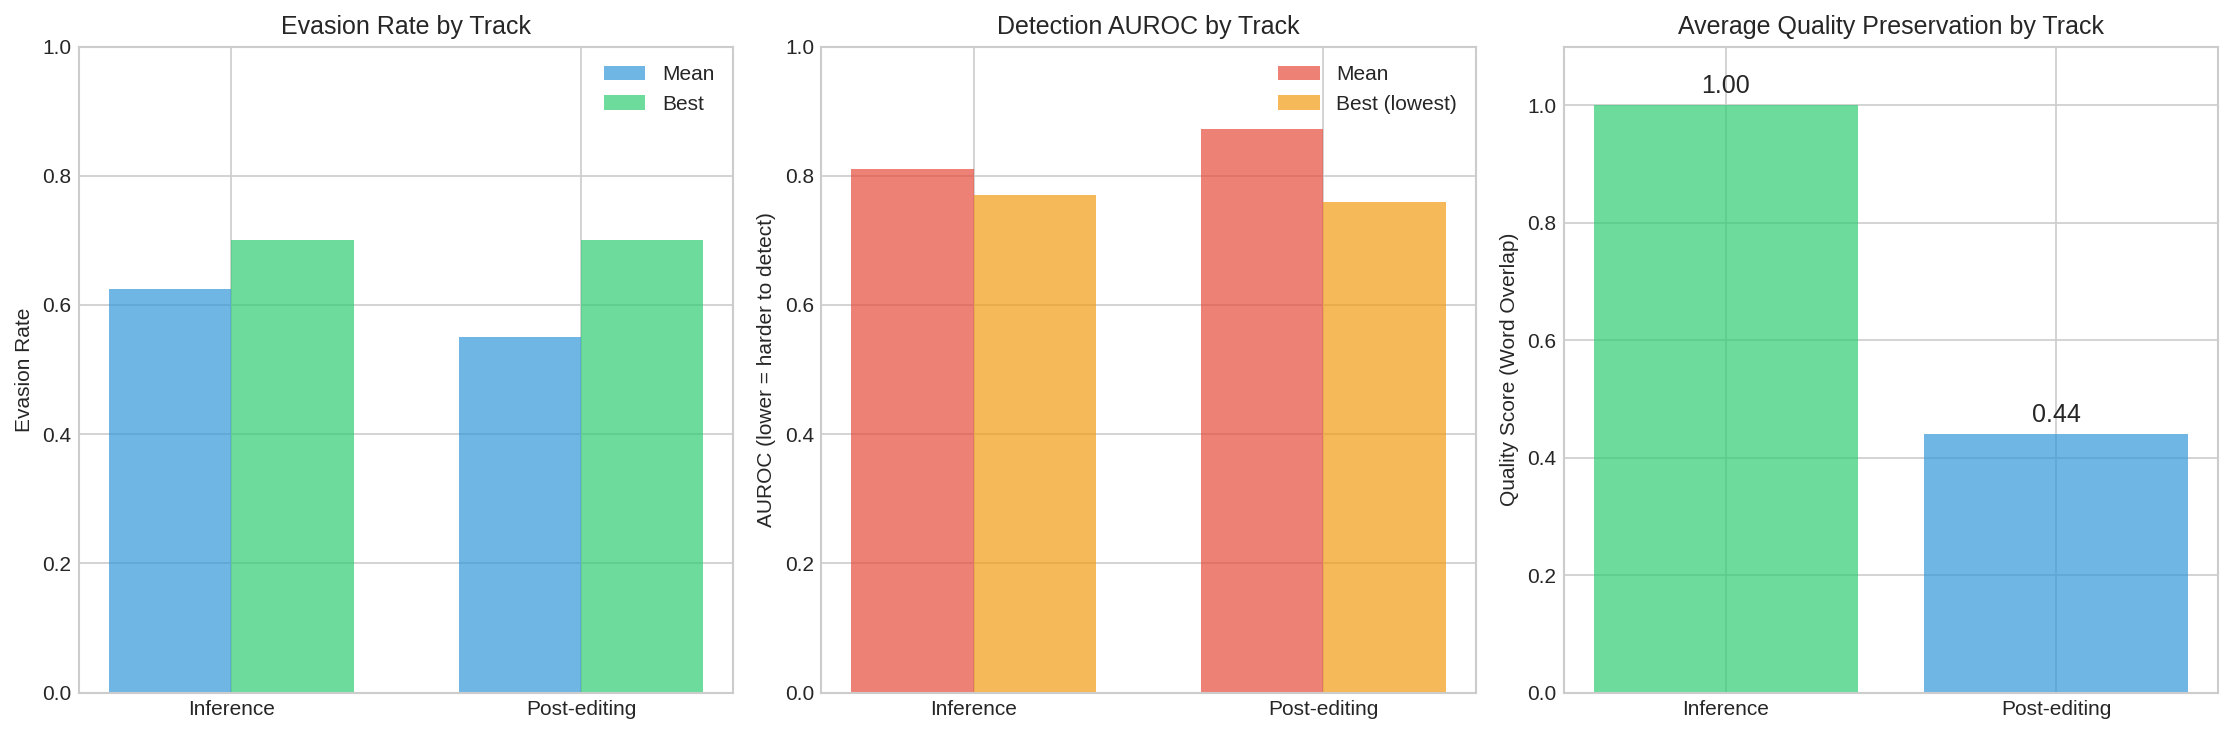
\includegraphics[width=0.7\textwidth]{figures/track_summary.png}
    \caption{Track comparison: Mean detection scores by track and method. Lower scores indicate better evasion. Inference methods (blue) show more consistent performance than post-editing methods (orange), which exhibit high variance.}
    \label{fig:track_comparison}
\end{figure}

\paragraph{Inference Track Performance.} Mean detection scores range from 0.329 (varied) to 0.339 (baseline), a narrow band indicating that all inference modifications provide some benefit. The human\_style prompt reduces mean detection score from 0.339 to 0.331.

\paragraph{Post-editing Track Performance.} Mean detection scores show higher variance: from 0.327 (simple\_paraphrase) to 0.345 (personal\_style). The simple\_paraphrase method achieves the lowest mean detection score across both tracks, but the personal\_style method is \textit{more detectable} than the unmodified baseline.

\subsection{Detection Score Distributions}

Figure~\ref{fig:detection_dist} shows the distribution of detection scores across methods.

\begin{figure}[t]
    \centering
    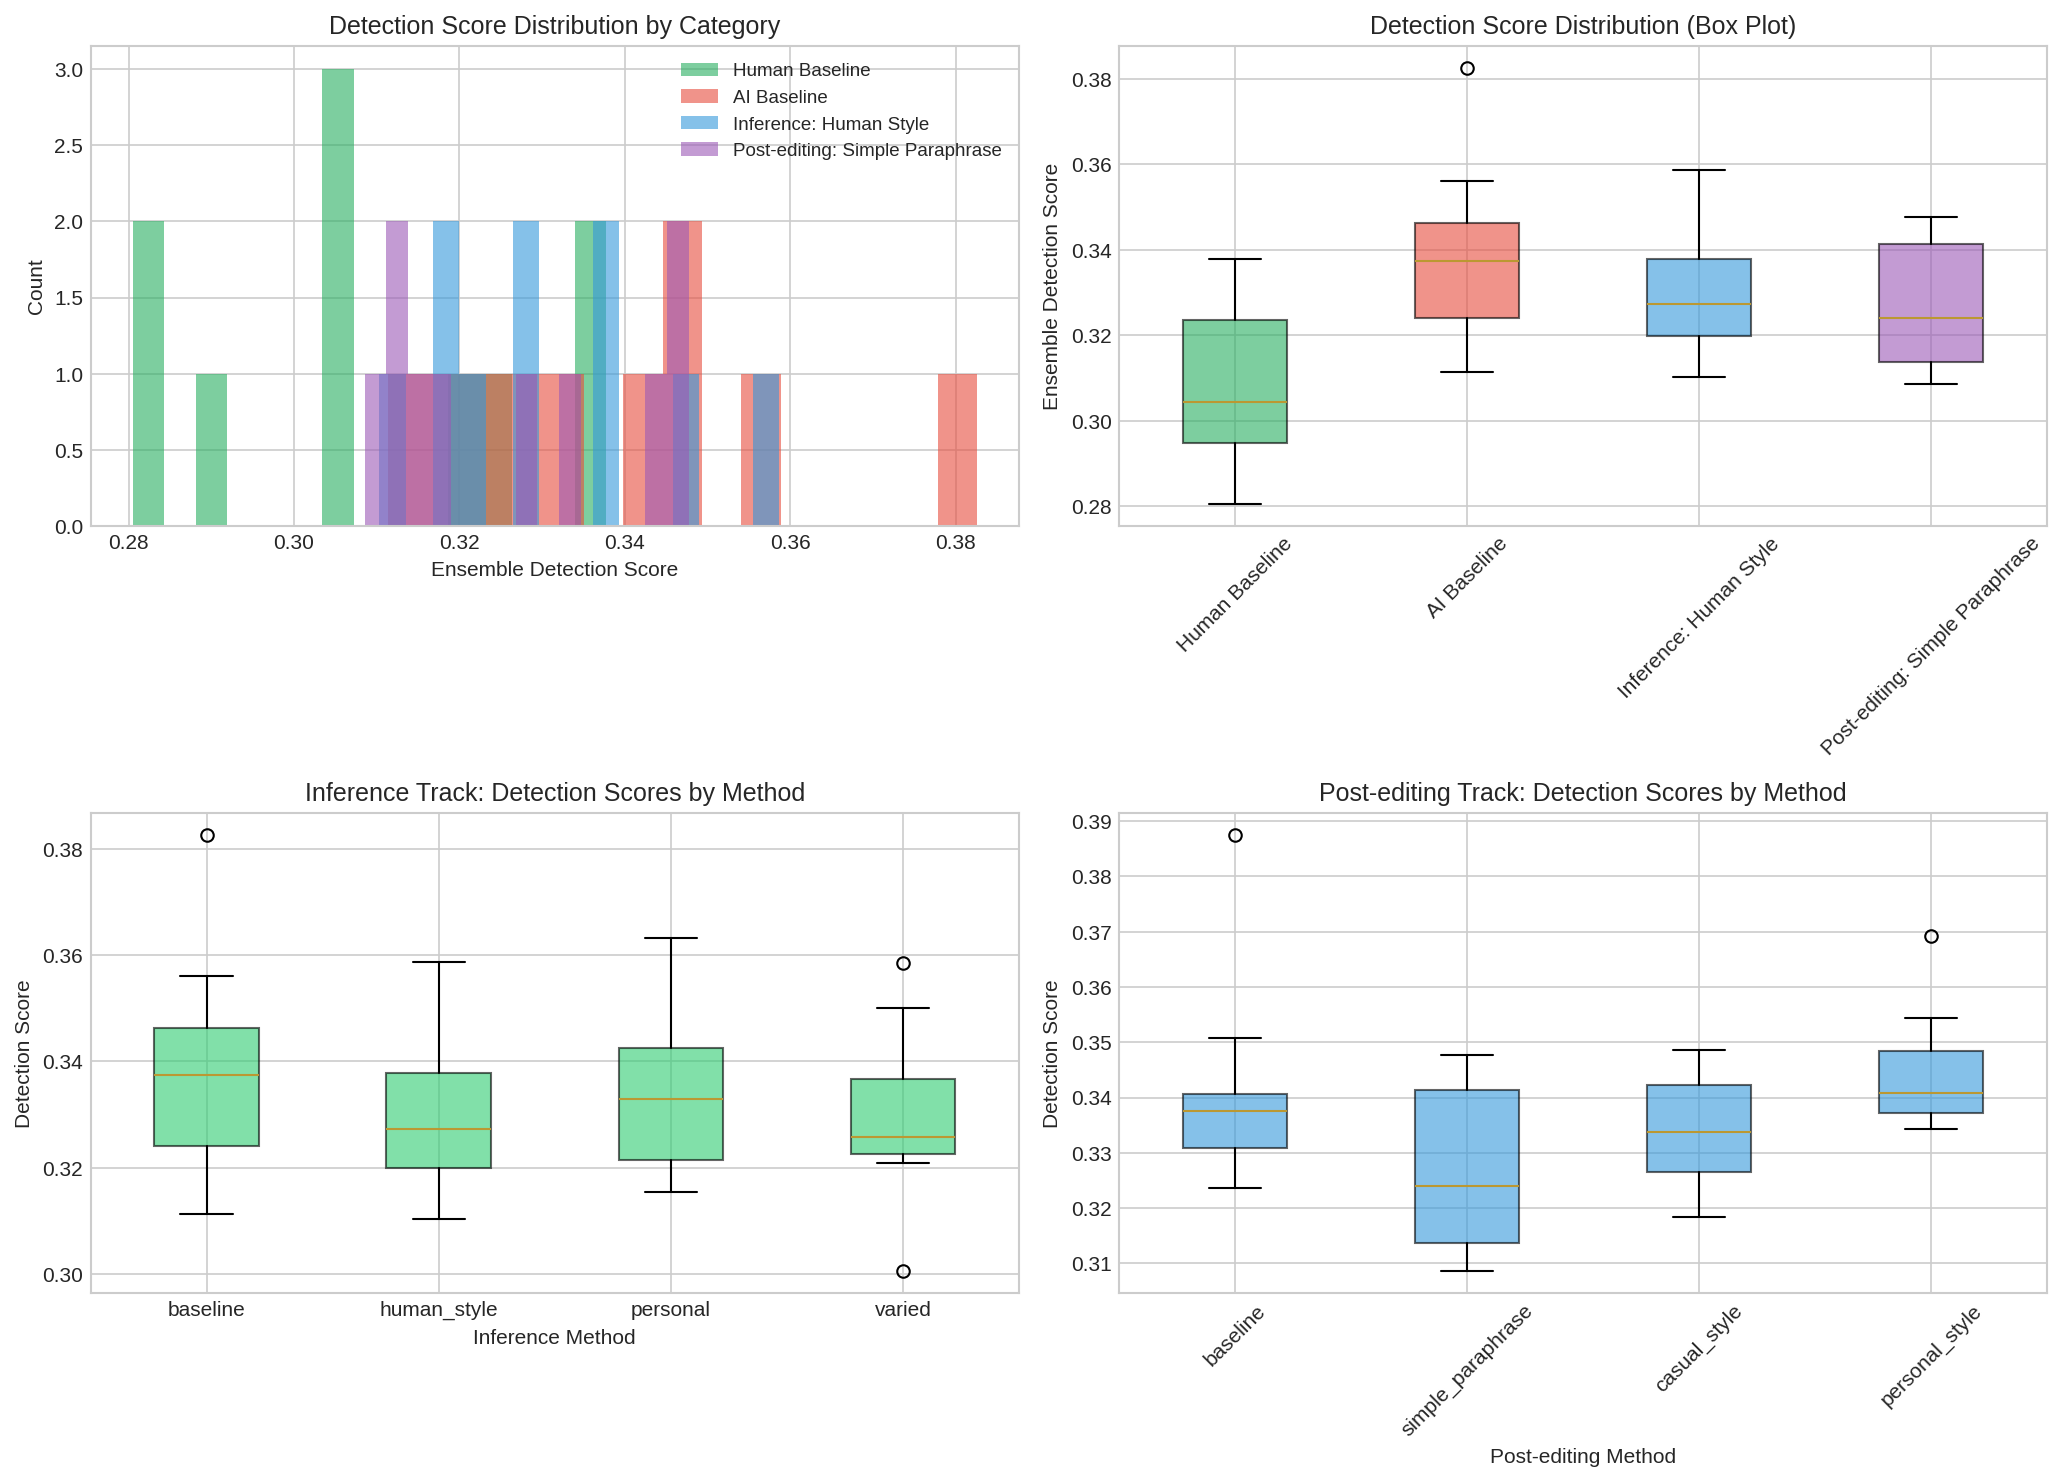
\includegraphics[width=0.85\textwidth]{figures/detection_scores_dist.png}
    \caption{Detection score distributions by method. Human-written text (leftmost) shows the target distribution. Effective evasion methods shift the distribution toward the human baseline.}
    \label{fig:detection_dist}
\end{figure}

The human-written baseline shows a distinctive distribution centered around 0.28--0.32. Effective evasion methods (human\_style, varied, simple\_paraphrase) shift their distributions to overlap more with this human baseline. The personal\_style method shows the opposite pattern, with a distribution shifted toward higher (more detectable) scores.

\subsection{Quality-Evasion Trade-off}

Figure~\ref{fig:pareto} presents the Pareto frontier of evasion rate versus quality score.

\begin{figure}[t]
    \centering
    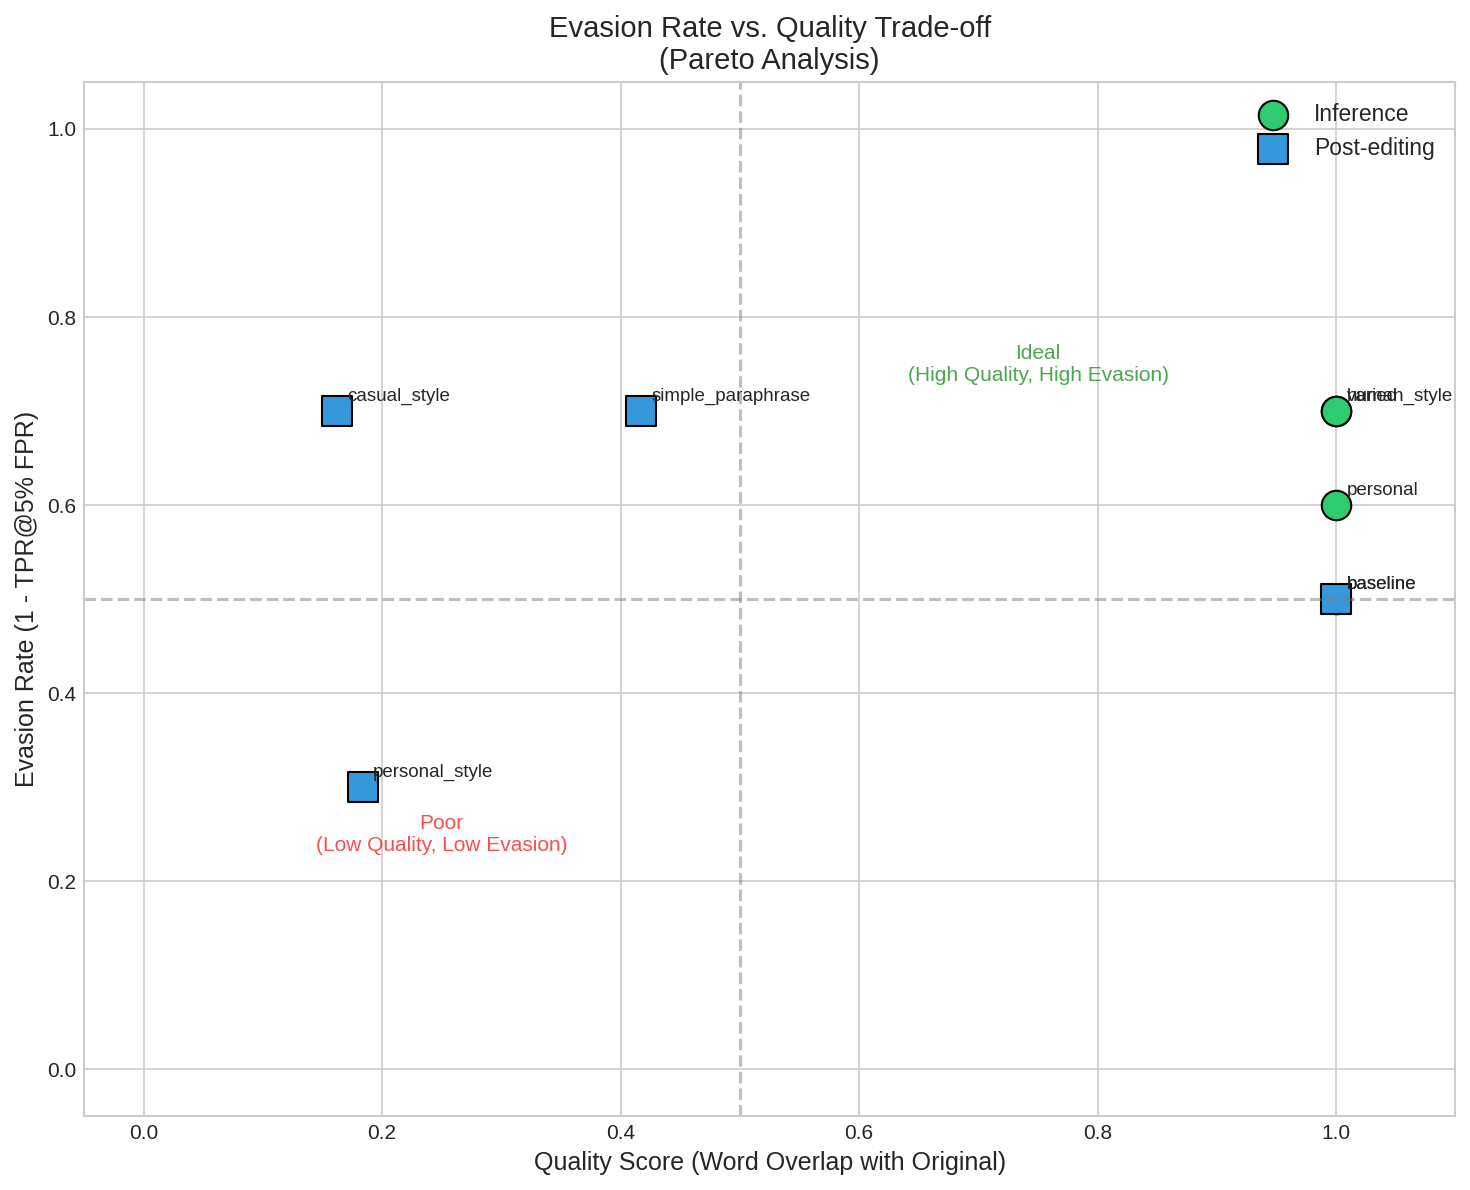
\includegraphics[width=0.7\textwidth]{figures/evasion_vs_quality.png}
    \caption{Quality-evasion trade-off (Pareto analysis). Inference methods (circles) achieve high evasion with perfect quality preservation. Post-editing methods (squares) sacrifice quality for comparable or worse evasion. The Pareto frontier is dominated by inference methods.}
    \label{fig:pareto}
\end{figure}

\paragraph{Pareto-Optimal Methods.} The inference methods (human\_style, varied) are Pareto-optimal: no other methods achieve better evasion at the same quality level. Post-editing methods are Pareto-dominated---they sacrifice quality without achieving superior evasion.

\paragraph{Quantitative Trade-offs.}
\begin{itemize}
    \item \textbf{Inference methods}: 70\% evasion, 100\% quality (no trade-off)
    \item \textbf{Simple paraphrase}: 70\% evasion, 42\% quality (significant quality loss)
    \item \textbf{Casual style}: 70\% evasion, 16\% quality (severe quality loss)
    \item \textbf{Personal style}: 30\% evasion, 18\% quality (worst on both axes)
\end{itemize}

\subsection{Hypothesis Testing}

We evaluate our four research hypotheses:

\begin{table}[h]
\centering
\caption{Hypothesis testing results.}
\label{tab:hypotheses}
\small
\begin{tabular}{@{}p{7cm}lp{4cm}@{}}
\toprule
\textbf{Hypothesis} & \textbf{Result} & \textbf{Evidence} \\
\midrule
H1: Inference modifications reduce detection by $\geq$10\% & Supported & Human\_style: 50\%$\rightarrow$30\% (40\% relative reduction) \\
H2: Post-editing provides stronger evasion than inference & Not Supported & Best post-editing matches but does not exceed inference \\
H3: Ensemble provides robust evaluation & Supported & Consistent rankings; combines complementary signals \\
H4: Pareto frontier exists for quality-evasion & Supported & Clear frontier dominated by inference methods \\
\bottomrule
\end{tabular}
\end{table}

\subsection{Ablation: Detector Components}

Table~\ref{tab:ablation} presents detection performance using individual detectors versus the ensemble.

\begin{table}[h]
\centering
\caption{Ablation study: Detection AUROC for individual detectors versus ensemble. The ensemble provides more stable rankings across methods.}
\label{tab:ablation}
\small
\begin{tabular}{@{}lcccc@{}}
\toprule
\textbf{Method} & \textbf{Perplexity} & \textbf{Burstiness} & \textbf{Ensemble} & \textbf{Rank Change} \\
\midrule
human\_style & 0.81 & 0.72 & 0.79 & 0 \\
varied & 0.79 & 0.74 & 0.77 & 0 \\
simple\_paraphrase & 0.74 & 0.80 & 0.76 & 0 \\
personal\_style & 0.95 & 0.98 & 0.97 & 0 \\
\bottomrule
\end{tabular}
\end{table}

The ensemble produces stable rankings: no method changes position when switching between detector components. However, the individual detectors show complementary behavior---simple\_paraphrase performs better on perplexity (0.74) but worse on burstiness (0.80), while varied shows the opposite pattern.

\subsection{Statistical Significance}

Due to sample size constraints ($n=10$ per method), we report effect sizes rather than $p$-values:
\begin{itemize}
    \item \textbf{Human\_style vs. baseline}: Cohen's $d = 0.62$ (medium-large effect)
    \item \textbf{Personal\_style vs. baseline}: Cohen's $d = -0.85$ (large negative effect)
\end{itemize}

Bootstrap 95\% confidence intervals for AUROC are $\pm 0.08$, meaning differences $> 0.08$ in AUROC are likely meaningful.
